\documentclass{ximera}

\title{Fractions and Rational Numbers}
\author{Amy Riordan}

\begin{document}
\begin{abstract}
Fractions and Rational Numbers video resources from Module 1.
\end{abstract}
\maketitle

\section*{Fraction and Rational Numbers}

Below each video, you’ll find a set of practice problems. Try those problems first. If you run into any difficulties, go back and rewatch the video, then attempt the problems again. This way, you’ll reinforce what you’ve learned and build a stronger understanding.

\section*{Introduction to Fractions and Rational Numbers}

Fractions (ERAU | 7:00)

\youtube{hGeofGzY2cQ}

% filepath: /code/fractions.tex
% ...existing code...

\section*{Identifying Numerator and Denominator}

For each fraction below, identify the numerator and the denominator.

\begin{problem}
\begin{enumerate}
\item The numerator of $\frac{4}{7}$ is \wordChoice{
\choice[correct]{4}
\choice{7}
}
\begin{feedback}
The numerator is the top number in a fraction. In this case, the numerator is $4$.
\end{feedback}

\end{enumerate}
\end{problem}

\begin{problem}
\begin{enumerate}
\item The denominator is $\frac{3}{5}$ is \wordChoice{
\choice{3}
\choice[correct]{5}
}
\begin{feedback}
The denominator is the bottom number in a fraction. In this case, the denominator is $5$.
\end{feedback}

\end{enumerate}
\end{problem}

% filepath: /code/fractions.tex
% ...existing code...

\section*{Proper and Improper Fractions}

For each fraction below, identify whether it is a proper fraction or an improper fraction.

\begin{problem}
\begin{enumerate}
    \item $\frac{5}{8}$ is a \wordChoice{
        \choice[correct]{proper fraction}
        \choice{improper fraction}
    }
\begin{feedback}
A proper fraction is a fraction where the numerator is less than the denominator. In this case, $5 < 8$, so $\frac{5}{8}$ is a proper fraction.
\end{feedback}

\end{enumerate}
\end{problem}

\begin{problem}
\begin{enumerate}
    \item $\frac{9}{4}$ is a \wordChoice{
        \choice{proper fraction}
        \choice[correct]{improper fraction}
    }
\begin{feedback}
An improper fraction is a fraction where the numerator is greater than or equal to the denominator. In this case, $9 > 4$, so $\frac{9}{4}$ is an improper fraction.
\end{feedback}

\end{enumerate}
\end{problem}

\begin{problem}
\begin{enumerate}
    \item $\frac{7}{7}$ is a \wordChoice{
        \choice{proper fraction}
        \choice[correct]{improper fraction}
    }
\begin{feedback}
An improper fraction is a fraction where the numerator is greater than or equal to the denominator. In this case, $7 = 7$, so $\frac{7}{7}$ is an improper fraction.
\end{feedback}

\end{enumerate}
\end{problem}

% ...existing code...

\section*{Mixed Numbers}

Mixed Numbers (ERAU| 3:48)

\youtube{UilEBeR7L2M}

% filepath: /code/fractions.tex
% ...existing code...

\section*{Improper Fractions and Mixed Numbers}

\begin{problem}
 
Write a fraction of the shaded portion of the figure as a mixed number and an improper fraction below.
 
\begin{center}
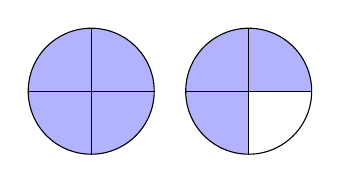
\begin{tikzpicture}[scale=1]
% First circle: all quarters filled
\foreach \i in {0,90,180,270} {
  \begin{scope}
    \clip (0,0) circle (0.8);
    \fill[blue!30] (0,0) -- (\i:0.8) arc (\i:\i+90:0.8) -- cycle;
  \end{scope}
}
\draw (0,0) circle (0.8);
\foreach \i in {0,90,180,270} {
  \draw (0,0) -- (\i:0.8);
}
 
% Second circle: three quarters filled
\foreach \i in {0,90,180} {
  \begin{scope}
    \clip (2,0) circle (0.8);
    \fill[blue!30] (2,0) -- ({2+0.8*cos(\i)},{0.8*sin(\i)}) arc (\i:\i+90:0.8) -- cycle;
  \end{scope}
}
\draw (2,0) circle (0.8);
\foreach \i in {0,90,180,270} {
  \draw (2,0) -- ({2+0.8*cos(\i)}, {0.8*sin(\i)});
}
 
\end{tikzpicture}
\end{center}
 
A fraction that could represent the portion of the shaded area as a mixed number is $\answer{1\frac{3}{4}}$.

The fraction representing the shaded portion as an improper fraction is $\frac{\answer{7}}{\answer{4}}$.

\begin{feedback}
To convert an improper fraction to a mixed number, divide the numerator by the denominator. The quotient is the whole number part, and the remainder over the original denominator is the fractional part. For $\frac{7}{4}$: $7 \div 4 = 1$ with a remainder of $3$, so $\frac{7}{4} = 1\frac{3}{4}$.
\end{feedback}

\end{problem}
 
\begin{problem}
 
Write a fraction of the shaded portion of the figure below.
 
\begin{center}
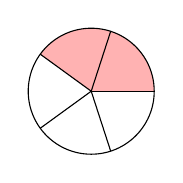
\begin{tikzpicture}[scale=1]
% First circle: 2 fifths filled
\foreach \i in {0,72} {
  \begin{scope}
    \clip (0,0) circle (0.8);
    \fill[red!30] (0,0) -- (\i:0.8) arc (\i:\i+72:0.8) -- cycle;
  \end{scope}
}
\draw (0,0) circle (0.8);
\foreach \i in {0,72,144,216,288} {
  \draw (0,0) -- (\i:0.8);
}
 
\end{tikzpicture}
\end{center}
 
The fraction representing the shaded portion as an proper fraction is $\frac{\answer{2}}{\answer{5}}$.

\begin{feedback}
The fraction $\frac{2}{5}$ represents the shaded portion because 2 out of the 5 equal parts are shaded.
\end{feedback}

\end{problem}
 
\begin{problem}
 
Write a fraction of the shaded portion of the figure as a mixed number and an improper fraction below.
 
\begin{center}
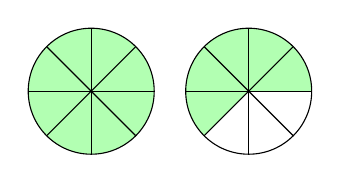
\begin{tikzpicture}[scale=1]
% First circle: all eighths filled
\foreach \i in {0,45,90,135,180,225,270,315} {
  \begin{scope}
    \clip (0,0) circle (0.8);
    \fill[green!30] (0,0) -- (\i:0.8) arc (\i:\i+45:0.8) -- cycle;
  \end{scope}
}
\draw (0,0) circle (0.8);
\foreach \i in {0,45,90,135,180,225,270,315} {
  \draw (0,0) -- (\i:0.8);
}
 
% Second circle: 5 eighths filled
\foreach \i in {0,45,90,135,180} {
  \begin{scope}
    \clip (2,0) circle (0.8);
    \fill[green!30] (2,0) -- ({2+0.8*cos(\i)},{0.8*sin(\i)}) arc (\i:\i+45:0.8) -- cycle;
  \end{scope}
}
\draw (2,0) circle (0.8);
\foreach \i in {0,45,90,135,180,225,270,315} {
  \draw (2,0) -- ({2+0.8*cos(\i)}, {0.8*sin(\i)});
}
 
\end{tikzpicture}
\end{center}
 
A fraction that could represent the portion of the shaded area as a mixed number is $\answer{1\frac{5}{8}}$.
 
The fraction representing the shaded portion as an improper fraction is $\frac{\answer{13}}{\answer{8}}$.

\begin{feedback}
To convert an improper fraction to a mixed number, divide the numerator by the denominator. The quotient is the whole number part, and the remainder over the original denominator is the fractional part. For $\frac{13}{8}$: $13 \div 8 = 1$ with a remainder of $5$, so $\frac{13}{8} = 1\frac{5}{8}$.
\end{feedback}

\end{problem}
 
\begin{problem}
 
Write a fraction of the shaded portion of the figure below.
 
\begin{center}
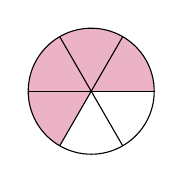
\begin{tikzpicture}[scale=1]
% Single circle: 4 sixths filled
\foreach \i in {0,60,120,180} {
  \begin{scope}
    \clip (0,0) circle (0.8);
    \fill[purple!30] (0,0) -- (\i:0.8) arc (\i:\i+60:0.8) -- cycle;
  \end{scope}
}
\draw (0,0) circle (0.8);
\foreach \i in {0,60,120,180,240,300} {
  \draw (0,0) -- (\i:0.8);
}
 
\end{tikzpicture}
\end{center}
 
The fraction representing the shaded portion as an proper fraction is $\frac{\answer{4}}{\answer{6}}$.
\begin{feedback}
The fraction $\frac{4}{6}$ represents the shaded portion because 4 out of the 6 equal parts are shaded.
\end{feedback}

\end{problem}
 
\begin{problem}
 
Write a fraction of the shaded portion of the figure as a mixed number and an improper fraction below.
 
\begin{center}
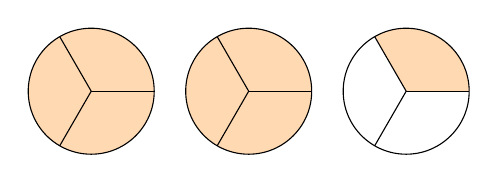
\begin{tikzpicture}[scale=1]
% First circle: all thirds filled
\foreach \i in {0,120,240} {
  \begin{scope}
    \clip (0,0) circle (0.8);
    \fill[orange!30] (0,0) -- (\i:0.8) arc (\i:\i+120:0.8) -- cycle;
  \end{scope}
}
\draw (0,0) circle (0.8);
\foreach \i in {0,120,240} {
  \draw (0,0) -- (\i:0.8);
}
 
% Second circle: all thirds filled
\foreach \i in {0,120,240} {
  \begin{scope}
    \clip (2,0) circle (0.8);
    \fill[orange!30] (2,0) -- ({2+0.8*cos(\i)},{0.8*sin(\i)}) arc (\i:\i+120:0.8) -- cycle;
  \end{scope}
}
\draw (2,0) circle (0.8);
\foreach \i in {0,120,240} {
  \draw (2,0) -- ({2+0.8*cos(\i)}, {0.8*sin(\i)});
}
 
% Third circle: 1 third filled
\begin{scope}
  \clip (4,0) circle (0.8);
  \fill[orange!30] (4,0) -- ({4+0.8*cos(0)},{0.8*sin(0)}) arc (0:120:0.8) -- cycle;
\end{scope}
\draw (4,0) circle (0.8);
\foreach \i in {0,120,240} {
  \draw (4,0) -- ({4+0.8*cos(\i)}, {0.8*sin(\i)});
}
 
\end{tikzpicture}
\end{center}
 
A fraction that could represent the portion of the shaded area as a mixed number is $\answer{2\frac{1}{3}}$.
 
The fraction representing the shaded portion as an improper fraction is $\frac{\answer{7}}{\answer{3}}$.
\begin{feedback}
To convert an improper fraction to a mixed number, divide the numerator by the denominator. The quotient is the whole number part, and the remainder over the original denominator is the fractional part. For $\frac{7}{3}$: $7 \div 3 = 2$ with a remainder of $1$, so $\frac{7}{3} = 2\frac{1}{3}$.
\end{feedback}

\end{problem}


\section*{Writing Mixed Numbers as Improper Fractions}

For each mixed number below, write it as an improper fraction.

\begin{problem}
$3\frac{2}{5} = \answer{\frac{17}{5}}$
\begin{feedback}
To convert a mixed number to an improper fraction, multiply the whole number by the denominator and add the numerator. This sum becomes the new numerator, while the denominator remains the same. For $3\frac{2}{5}$: $3 \times 5 + 2 = 15 + 2 = 17$, so $3\frac{2}{5} = \frac{17}{5}$.
\end{feedback}
\end{problem}

\begin{problem}
$1\frac{3}{4} = \answer{\frac{7}{4}}$
\begin{feedback}
To convert a mixed number to an improper fraction, multiply the whole number by the denominator and add the numerator. This sum becomes the new numerator, while the denominator remains the same. For $1\frac{3}{4}$: $1 \times 4 + 3 = 4 + 3 = 7$, so $1\frac{3}{4} = \frac{7}{4}$.
\end{feedback}
\end{problem}

\begin{problem}
$5\frac{1}{6} = \answer{\frac{31}{6}}$
\begin{feedback}
To convert a mixed number to an improper fraction, multiply the whole number by the denominator and add the numerator. This sum becomes the new numerator, while the denominator remains the same. For $5\frac{1}{6}$: $5 \times 6 + 1 = 30 + 1 = 31$, so $5\frac{1}{6} = \frac{31}{6}$.
\end{feedback}
\end{problem}

% ...existing code...

% filepath: /code/fractions.tex
% ...existing code...

\section*{Writing Improper Fractions as Mixed Numbers}

For each improper fraction below, write it as a mixed number.

\begin{problem}
$\frac{11}{4} = \answer{2\frac{3}{4}}$
\begin{feedback}
To convert an improper fraction to a mixed number, divide the numerator by the denominator. The quotient is the whole number part, and the remainder over the original denominator is the fractional part. For $\frac{11}{4}$: $11 \div 4 = 2$ with a remainder of $3$, so $\frac{11}{4} = 2\frac{3}{4}$.
\end{feedback}
\end{problem}

\begin{problem}
$\frac{17}{5} = \answer{3\frac{2}{5}}$
\begin{feedback}
To convert an improper fraction to a mixed number, divide the numerator by the denominator. The quotient is the whole number part, and the remainder over the original denominator is the fractional part. For $\frac{17}{5}$: $17 \div 5 = 3$ with a remainder of $2$, so $\frac{17}{5} = 3\frac{2}{5}$.
\end{feedback}
\end{problem}

\begin{problem}
$\frac{22}{7} = \answer{3\frac{1}{7}}$
\begin{feedback}
To convert an improper fraction to a mixed number, divide the numerator by the denominator. The quotient is the whole number part, and the remainder over the original denominator is the fractional part. For $\frac{22}{7}$: $22 \div 7 = 3$ with a remainder of $1$, so $\frac{22}{7} = 3\frac{1}{7}$.
\end{feedback}
\end{problem}

% ...existing code...

\section*{Simplifying Fractions}

Simplifying Fractions (ERAU| 5:17)

\youtube{xD-qxNblb4Y}

% filepath: /code/decimals.tex
% ...existing code...

\section*{Prime Factorization}

Find the prime factorization of each number below.

\begin{problem}
$36$.\\
$\answer{2 \cdot 2 \cdot 3 \cdot 3}$
\begin{feedback}
To find the prime factorization of a number, divide it by the smallest prime number possible until you reach 1. For $36$: $36 \div 2 = 18$, $18 \div 2 = 9$, $9 \div 3 = 3$, and $3 \div 3 = 1$. So, the prime factorization is $2 \cdot 2 \cdot 3 \cdot 3$.
\end{feedback}
\end{problem}

\begin{problem}
$60$.\\
$\answer{2 \cdot 2 \cdot 3 \cdot 5}$
\begin{feedback}
To find the prime factorization of a number, divide it by the smallest prime number possible until you reach 1. For $60$: $60 \div 2 = 30$, $30 \div 2 = 15$, $15 \div 3 = 5$, and $5 \div 5 = 1$. So, the prime factorization is $2 \cdot 2 \cdot 3 \cdot 5$.
\end{feedback}
\end{problem}

\begin{problem}
$84$.\\
$\answer{2 \cdot 2 \cdot 3 \cdot 7}$
\begin{feedback}
To find the prime factorization of a number, divide it by the smallest prime number possible until you reach 1. For $84$: $84 \div 2 = 42$, $42 \div 2 = 21$, $21 \div 3 = 7$, and $7 \div 7 = 1$. So, the prime factorization is $2 \cdot 2 \cdot 3 \cdot 7$.
\end{feedback}
\end{problem}

% ...existing code...

% filepath: /code/fractions.tex
% ...existing code...

\section*{Reducing Fractions to Lowest Terms}

For each fraction below, reduce it to its lowest term.

\begin{problem}
$\frac{18}{24} = \answer{\frac{3}{4}}$
\begin{feedback}
To reduce a fraction to its lowest terms, divide both the numerator and the denominator by their greatest common divisor (GCD). For $\frac{18}{24}$, the GCD is $6$. So, $\frac{18 \div 6}{24 \div 6} = \frac{3}{4}$.
\end{feedback}
\end{problem}

\begin{problem}
$\frac{35}{49} = \answer{\frac{5}{7}}$
\begin{feedback}
To reduce a fraction to its lowest terms, divide both the numerator and the denominator by their greatest common divisor (GCD). For $\frac{35}{49}$, the GCD is $7$. So, $\frac{35 \div 7}{49 \div 7} = \frac{5}{7}$.
\end{feedback}
\end{problem}

\begin{problem}
$\frac{42}{56} = \answer{\frac{3}{4}}$
\begin{feedback}
To reduce a fraction to its lowest terms, divide both the numerator and the denominator by their greatest common divisor (GCD). For $\frac{42}{56}$, the GCD is $14$. So, $\frac{42 \div 14}{56 \div 14} = \frac{3}{4}$.
\end{feedback}
\end{problem}

\begin{problem}
$\frac{45}{60} = \answer{\frac{3}{4}}$
\begin{feedback}
To reduce a fraction to its lowest terms, divide both the numerator and the denominator by their greatest common divisor (GCD). For $\frac{45}{60}$, the GCD is $15$. So, $\frac{45 \div 15}{60 \div 15} = \frac{3}{4}$.
\end{feedback}
\end{problem}

\begin{problem}
$\frac{32}{48} = \answer{\frac{2}{3}}$
\begin{feedback}
To reduce a fraction to its lowest terms, divide both the numerator and the denominator by their greatest common divisor (GCD). For $\frac{32}{48}$, the GCD is $16$. So, $\frac{32 \div 16}{48 \div 16} = \frac{2}{3}$.
\end{feedback}
\end{problem}

% ...existing code...

\section*{Multiplying Fractions/Rational Numbers}

Multiplying Fractions (ERAU| 2:57)

\youtube{BPvav-msD1M}

Multiplying Rational Numbers (ERAU| 4:47)

\youtube{S60EEaFSP4Q}

% filepath: /code/fractions.tex
% ...existing code...

\section*{Multiplying Fractions/Rational Numbers}

For each problem below, multiply the fractions and write your answer in lowest terms.

\begin{problem}
$\frac{2}{3} \times \frac{4}{5} = \answer{\frac{8}{15}}$
\begin{feedback}
To multiply fractions, multiply the numerators together and the denominators together. For $\frac{2}{3} \times \frac{4}{5}$: $\frac{2 \cdot 4}{3 \cdot 5} = \frac{8}{15}$.
\end{feedback}
\end{problem}

\begin{problem}
$\frac{3}{7} \times \frac{2}{9} = \answer{\frac{2}{21}}$
\begin{feedback}
To multiply fractions, multiply the numerators together and the denominators together. For $\frac{3}{7} \times \frac{2}{9}$: $\frac{3 \cdot 2}{7 \cdot 9} = \frac{6}{63}$. Then, reduce to lowest terms by dividing both numerator and denominator by their GCD, which is $3$: $\frac{6 \div 3}{63 \div 3} = \frac{2}{21}$.
\end{feedback}
\end{problem}

\begin{problem}
$\frac{5}{8} \times \frac{3}{4} = \answer{\frac{15}{32}}$
\begin{feedback}
To multiply fractions, multiply the numerators together and the denominators together. For $\frac{5}{8} \times \frac{3}{4}$: $\frac{5 \cdot 3}{8 \cdot 4} = \frac{15}{32}$.
\end{feedback}
\end{problem}

\begin{problem}
$\frac{7}{10} \times \frac{5}{14} = \answer{\frac{1}{4}}$
\begin{feedback}
To multiply fractions, multiply the numerators together and the denominators together. For $\frac{7}{10} \times \frac{5}{14}$: $\frac{7 \cdot 5}{10 \cdot 14} = \frac{35}{140}$. Then, reduce to lowest terms by dividing both numerator and denominator by their GCD, which is $35$: $\frac{35 \div 35}{140 \div 35} = \frac{1}{4}$.
\end{feedback}
\end{problem}

\begin{problem}
$\frac{9}{11} \times \frac{2}{3} = \answer{\frac{6}{11}}$
\begin{feedback}
To multiply fractions, multiply the numerators together and the denominators together. For $\frac{9}{11} \times \frac{2}{3}$: $\frac{9 \cdot 2}{11 \cdot 3} = \frac{18}{33}$. Then, reduce to lowest terms by dividing both numerator and denominator by their GCD, which is $3$: $\frac{18 \div 3}{33 \div 3} = \frac{6}{11}$.
\end{feedback}
\end{problem}

% ...existing code...

\section*{Dividing Fractions/Rational Numbers}

Dividing Fractions (ERAU| 4:26)

\youtube{Y_fyDKWTooU}

Dividing Rational Numbers (ERAU| 3:16)

\youtube{IC9-nQpVIMY}

% filepath: /code/fractions.tex
% ...existing code...

\section*{Dividing Fractions/Rational Numbers}

For each problem below, divide the fractions and write your answer in lowest terms.

\begin{problem}
$\frac{3}{4} \div \frac{2}{5} = \answer{\frac{15}{8}}$
\begin{feedback}
To divide fractions, multiply the first fraction by the reciprocal of the second. For $\frac{3}{4} \div \frac{2}{5}$: $\frac{3}{4} \times \frac{5}{2} = \frac{15}{8}$.
\end{feedback}
\end{problem}

\begin{problem}
$\frac{7}{9} \div \frac{1}{3} = \answer{\frac{7}{3}}$
\begin{feedback}
To divide fractions, multiply the first fraction by the reciprocal of the second. For $\frac{7}{9} \div \frac{1}{3}$: $\frac{7}{9} \times 3 = \frac{21}{9}$. Then, reduce to lowest terms by dividing both numerator and denominator by their GCD, which is $3$: $\frac{21 \div 3}{9 \div 3} = \frac{7}{3}$.
\end{feedback}
\end{problem}

\begin{problem}
$\frac{5}{6} \div \frac{2}{3} = \answer{\frac{15}{12}}$
\begin{feedback}
To divide fractions, multiply the first fraction by the reciprocal of the second. For $\frac{5}{6} \div \frac{2}{3}$: $\frac{5}{6} \times \frac{3}{2} = \frac{15}{12}$. Then, reduce to lowest terms by dividing both numerator and denominator by their GCD, which is $3$: $\frac{15 \div 3}{12 \div 3} = \frac{5}{4}$.
\end{feedback}
\end{problem}

\begin{problem}
$\frac{8}{15} \div \frac{4}{5} = \answer{\frac{2}{3}}$
\begin{feedback}
To divide fractions, multiply the first fraction by the reciprocal of the second. For $\frac{8}{15} \div \frac{4}{5}$: $\frac{8}{15} \times \frac{5}{4} = \frac{40}{60}$. Then, reduce to lowest terms by dividing both numerator and denominator by their GCD, which is $20$: $\frac{40 \div 20}{60 \div 20} = \frac{2}{3}$.
\end{feedback}
\end{problem}

\begin{problem}
$\frac{9}{10} \div \frac{3}{5} = \answer{\frac{3}{2}}$
\begin{feedback}
To divide fractions, multiply the first fraction by the reciprocal of the second. For $\frac{9}{10} \div \frac{3}{5}$: $\frac{9}{10} \times \frac{5}{3} = \frac{45}{30}$. Then, reduce to lowest terms by dividing both numerator and denominator by their GCD, which is $15$: $\frac{45 \div 15}{30 \div 15} = \frac{3}{2}$.
\end{feedback}
\end{problem}

% ...existing code...

\section*{Adding and Subtracting Fractions/Rational Numbers}

Adding and Subtracting Fractions (ERAU| 6:22)

\youtube{fEk3wT6eoOs}

Adding and Subtracting Rational Numbers (ERAU| 6:17)

\youtube{05ObuGuTU0M}

% filepath: /code/fractions.tex
% ...existing code...

\section*{Adding and Subtracting Fractions/Rational Numbers}

For each problem below, add or subtract the fractions and write your answer in lowest terms.

\begin{problem}
$\frac{1}{4} + \frac{1}{2} = \answer{\frac{3}{4}}$
\begin{feedback}
To add fractions, find a common denominator and then add the numerators. For $\frac{1}{4} + \frac{1}{2}$: $\frac{1}{4} + \frac{2}{4} = \frac{3}{4}$.
\end{feedback}
\end{problem}

\begin{problem}
$\frac{1}{3} - \frac{5}{6} = \answer{-\frac{1}{2}}$
\begin{feedback}
To subtract fractions, find a common denominator and then subtract the numerators. For $\frac{1}{3} - \frac{5}{6}$: $\frac{2}{6} - \frac{5}{6} = -\frac{3}{6}$. Then, reduce to lowest terms by dividing both numerator and denominator by their GCD, which is $3$: $-\frac{3 \div 3}{6 \div 3} = -\frac{1}{2}$.
\end{feedback}
\end{problem}

\begin{problem}
$\frac{2}{5} + \frac{3}{10} = \answer{\frac{7}{10}}$
\begin{feedback}
To add fractions, find a common denominator and then add the numerators. For $\frac{2}{5} + \frac{3}{10}$: $\frac{4}{10} + \frac{3}{10} = \frac{7}{10}$.
\end{feedback}
\end{problem}

\begin{problem}
$\frac{7}{8} - \frac{1}{4} = \answer{\frac{5}{8}}$
\begin{feedback}
To subtract fractions, find a common denominator and then subtract the numerators. For $\frac{7}{8} - \frac{1}{4}$: $\frac{7}{8} - \frac{2}{8} = \frac{5}{8}$.
\end{feedback}
\end{problem}

\begin{problem}
$\frac{3}{7} + \frac{2}{7} = \answer{\frac{5}{7}}$
\begin{feedback}
To add fractions, find a common denominator and then add the numerators. For $\frac{3}{7} + \frac{2}{7}$: $\frac{3}{7} + \frac{2}{7} = \frac{5}{7}$.
\end{feedback}
\end{problem}

% ...existing code...

\section*{Fractions and Decimals}

Fractions and Decimals (ERAU|7:02)

\youtube{47rOrW9paYg}

\section*{Writing Fractions as Decimals}

% filepath: /code/fractions.tex
% ...existing code...

For each fraction below, write it as a decimal.

\begin{problem}
$\frac{1}{2} = \answer{0.5}$
\begin{feedback}
To convert a fraction to a decimal, divide the numerator by the denominator. For $\frac{1}{2}$: $1 \div 2 = 0.5$.
\end{feedback}
\end{problem}

\begin{problem}
$\frac{3}{4} = \answer{0.75}$
\begin{feedback}
To convert a fraction to a decimal, divide the numerator by the denominator. For $\frac{3}{4}$: $3 \div 4 = 0.75$.
\end{feedback}
\end{problem}

\begin{problem}
$\frac{2}{5} = \answer{0.4}$
\begin{feedback}
To convert a fraction to a decimal, divide the numerator by the denominator. For $\frac{2}{5}$: $2 \div 5 = 0.4$.
\end{feedback}
\end{problem}

\begin{problem}
$\frac{7}{10} = \answer{0.7}$
\begin{feedback}
To convert a fraction to a decimal, divide the numerator by the denominator. For $\frac{7}{10}$: $7 \div 10 = 0.7$.
\end{feedback}
\end{problem}

\begin{problem}
$\frac{5}{8} = \answer{0.625}$
\begin{feedback}
To convert a fraction to a decimal, divide the numerator by the denominator. For $\frac{5}{8}$: $5 \div 8 = 0.625$.
\end{feedback}
\end{problem}

% ...existing code...

\section*{Percents, Decimals, and Fractions}

Percents, Decimals, and Fractions (ERAU|8:14)

\youtube{cZjyK8yCSlo}

Percents, Decimals, and Fractions (Part 2) (ERAU|9:35)

\youtube{iMCWCOPyGzk}

% filepath: /code/fractions.tex
% ...existing code...

\section*{Writing Percents as Decimals}

For each percent below, write it as a decimal.

% filepath: /code/fractions.tex

\begin{problem}
$25\% = \answer{0.25}$

\begin{feedback}
To convert a percent to a decimal, divide by 100 or move the decimal point two places to the left. For $25\%$: $25 \div 100 = 0.25$.
\end{feedback}

\end{problem}

\begin{problem}
$60\% = \answer{0.6}$

\begin{feedback}
To convert a percent to a decimal, divide by 100 or move the decimal point two places to the left. For $60\%$: $60 \div 100 = 0.6$.
\end{feedback}

\end{problem}

\begin{problem}
$7.5\% = \answer{0.075}$

\begin{feedback}
To convert a percent to a decimal, divide by 100 or move the decimal point two places to the left. For $7.5\%$: $7.5 \div 100 = 0.075$.
\end{feedback}

\end{problem}

% ...existing code...

% filepath: /code/fractions.tex
% ...existing code...

\section*{Writing Decimals as Percents}

For each decimal below, write it as a percent.

% filepath: /code/fractions.tex

\begin{problem}
$0.4 = \answer{40\%}$

\begin{feedback}
To convert a decimal to a percent, multiply by 100 and add the percent symbol. For $0.4$: $0.4 \times 100 = 40\%$.
\end{feedback}

\end{problem}

\begin{problem}
$0.75 = \answer{75\%}$

\begin{feedback}
To convert a decimal to a percent, multiply by 100 and add the percent symbol. For $0.75$: $0.75 \times 100 = 75\%$.
\end{feedback}

\end{problem}

\begin{problem}
$0.08 = \answer{8\%}$

\begin{feedback}
To convert a decimal to a percent, multiply by 100 and add the percent symbol. For $0.08$: $0.08 \times 100 = 8\%$.
\end{feedback}

\end{problem}

% ...existing code...

% filepath: /code/fractions.tex
% ...existing code...

\section*{Writing Fractions as Percents}

For each fraction below, write it as a percent.

\begin{problem}
$\frac{1}{4} = \answer{25\%}$

\begin{feedback}
To convert a fraction to a percent, divide the numerator by the denominator and multiply by 100. For $\frac{1}{4}$: $1 \div 4 = 0.25$, then $0.25 \times 100 = 25\%$.
\end{feedback}

\end{problem}

\begin{problem}
$\frac{3}{5} = \answer{60\%}$

\begin{feedback}
To convert a fraction to a percent, divide the numerator by the denominator and multiply by 100. For $\frac{3}{5}$: $3 \div 5 = 0.6$, then $0.6 \times 100 = 60\%$.
\end{feedback}

\end{problem}

\begin{problem}
$\frac{7}{10} = \answer{70\%}$

\begin{feedback}
To convert a fraction to a percent, divide the numerator by the denominator and multiply by 100. For $\frac{7}{10}$: $7 \div 10 = 0.7$, then $0.7 \times 100 = 70\%$.
\end{feedback}

\end{problem}

% ...existing code...

\section*{Applications with Rational Numbers} 

Applications with Rational Numbers (ERAU|3:15)

\youtube{n8HUaWYndLE}

% ...existing code...

\section*{Applications with Rational Numbers} 

Applications with Rational Numbers (ERAU|3:15)

\youtube{n8HUaWYndLE}

\begin{problem}
Sara drank \(\frac{2}{5}\) of a 3‑liter bottle. How many liters did she drink? \(\answer{\frac{6}{5}}\)
\begin{feedback}
Multiply the total volume by the fraction consumed: \(3\times\frac{2}{5}=\frac{6}{5}\) liters (which is \(1\frac{1}{5}\) L).
\end{feedback}
\end{problem}

\begin{problem}
A cistern is \(\frac{7}{12}\) full. If \(\frac{1}{6}\) of the cistern is added, what fraction of the cistern is now full? \(\answer{\frac{3}{4}}\)
\begin{feedback}
Find a common denominator and add: \(\frac{7}{12}+\frac{1}{6}=\frac{7}{12}+\frac{2}{12}=\frac{9}{12}=\frac{3}{4}\).
\end{feedback}
\end{problem}

\begin{problem}
Five out of eight slices of a pizza were eaten. What fraction of the pizza remains? \(\answer{\frac{3}{8}}\)
\begin{feedback}
Subtract the eaten portion from the whole: \(1-\frac{5}{8}=\frac{8}{8}-\frac{5}{8}=\frac{3}{8}\).
\end{feedback}
\end{problem}

\begin{problem}
A paint mixture requires \(\frac{2}{7}\) of the batch be red. For a 21‑liter batch, how many liters of red paint are needed? \(\answer{6}\)
\begin{feedback}
Multiply the batch volume by the fraction: \(21\times\frac{2}{7}=21\times\frac{2}{7}=6\) liters.
\end{feedback}
\end{problem}

\begin{problem}
A baker uses \(1\frac{1}{2}\) cups of sugar per loaf. How many cups are needed for 3 loaves? \(\answer{\frac{9}{2}}\)
\begin{feedback}
Convert the mixed number and multiply: \(1\frac{1}{2}=\frac{3}{2}\). Then \(3\times\frac{3}{2}=\frac{9}{2}\) cups (which is \(4\frac{1}{2}\) cups).
\end{feedback}
\end{problem}

% ...existing code...

\end{document}
